\section{Aquisição}
\label{sec:aquisicao}

% fonte: notas/t1_metadados.md (ffprobe de cozinha.MOV)
\textbf{Captura.} A cozinha foi gravada em 30/10/2026 com um iPhone 14 Pro Max, na horizontal, em HEVC (High Efficiency Video Coding), 1920\,$\times$\,1080\,px, 30\,fps, 775,5\,s e 23262 quadros. A extração toma um quadro a cada 10, ou seja 3\,fps, sem redimensionar, e gera 2327 imagens, das quais 2326 foram registradas, 99,96\%. A câmera percorreu o ambiente à mão e fechou o laço em 76,13\,m de trajeto estimado.

\textbf{Desafios.} Há paredes lisas, vidros e contraluz. A análise de qualidade marca 730 dos 2327 quadros, mas nenhum é removido. Os motivos se sobrepõem: 524 quadros têm desfoque relativo, 181 saturação, 82 pouca textura e 56 pouco contraste. % fonte: frame_quality_metrics.csv
Foco e exposição do iPhone não são verificáveis, e não há marcador de escala: a escala vem do contorno medido (Seção~\ref{sec:metodo}).

\textbf{Medidas de referência.} Em 25/10/2026, no mesmo ambiente, o app Medida do iPhone deu cinco paredes (Figura~\ref{fig:medidas} e Tabela~\ref{tab:erro}). As medidas do app têm resolução de 1\,cm e foram feitas sobre a moldura do teto. % fonte: configs/measurements/kitchen_my_home.yaml
A altura, ou pé-direito, ainda não foi medida no local.

\begin{figure}[!htbp]
\centering
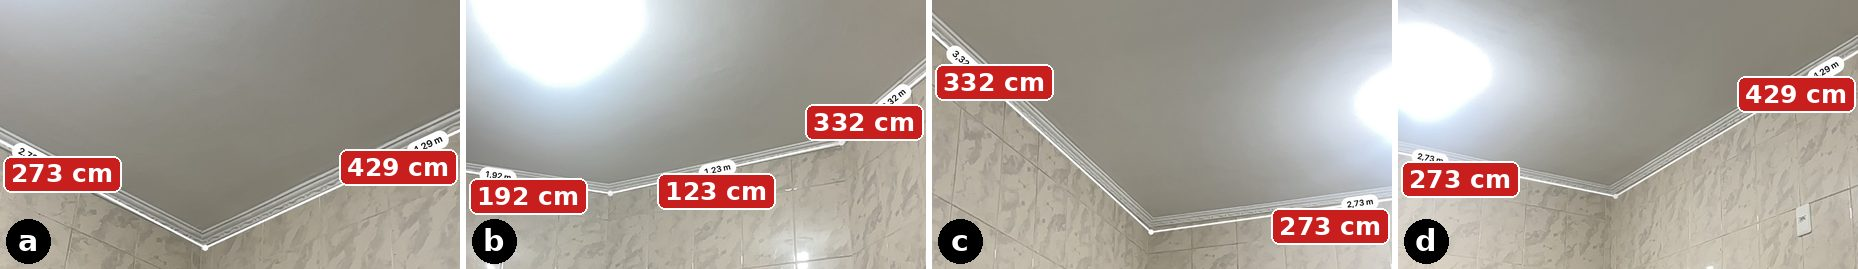
\includegraphics[width=\textwidth]{images/report/medidas.jpg}
\caption{Medidas de referência (app Medida do iPhone sobre a moldura do teto), em cm. Perímetro 13,49\,m, área 11,26\,m$^2$; pé-direito não medido.}
\label{fig:medidas}
\end{figure}
